\section{Evaluation}\label{sec:evaluation} 
In this chapter, I am going to evaluate the outcome of my thesis i.e. research and implementation work. 
Figure~\ref{fig:Evaluation_Phases} shows the phases of the entire evaluation process. Section \ref{subsec:goals} describes the research and case study phase. Section \ref{subsec:designmethod} illustrates the evaluation design method that I have used for conducting the experiment. This is then followed by a brief description about the planning phase in Section \ref{subsec:planning}. Afterwards, Section \ref{subsec:investigationgoals} deals with the formulas to investigate the goals of the evaluation process. Then, Section \ref{subsec:execution} describes the preparation and test execution phase in detail. Section \ref{subsec:threats&mitigation} explains the associated threats with the evaluation process and their mitigation criteria. At last, Section \ref{subsec:results} discusses the result generated from the gathered data. 

The aim of this chapter is as follows: 

\textbf{"Analyse the outcome of the usage of an interactive demonstrator for the purpose of evaluation with respect to the user from the point of view of the researcher in the context of spreading the basic concepts of bidirectional transformation (bx) and making them understandable and accessible."}

\subsection{Goals}\label{subsec:goals}  
In any research, there could be many cases and each case could focus on a number of different research questions, each of which leads to a different direction in developing solution strategies~\cite{semethods}. Hence, for any evaluation process, most important thing are selecting cases that are most relevant to the research and narrowing down the research questions only associated with the exact problems in hand. 

\begin{figure}
	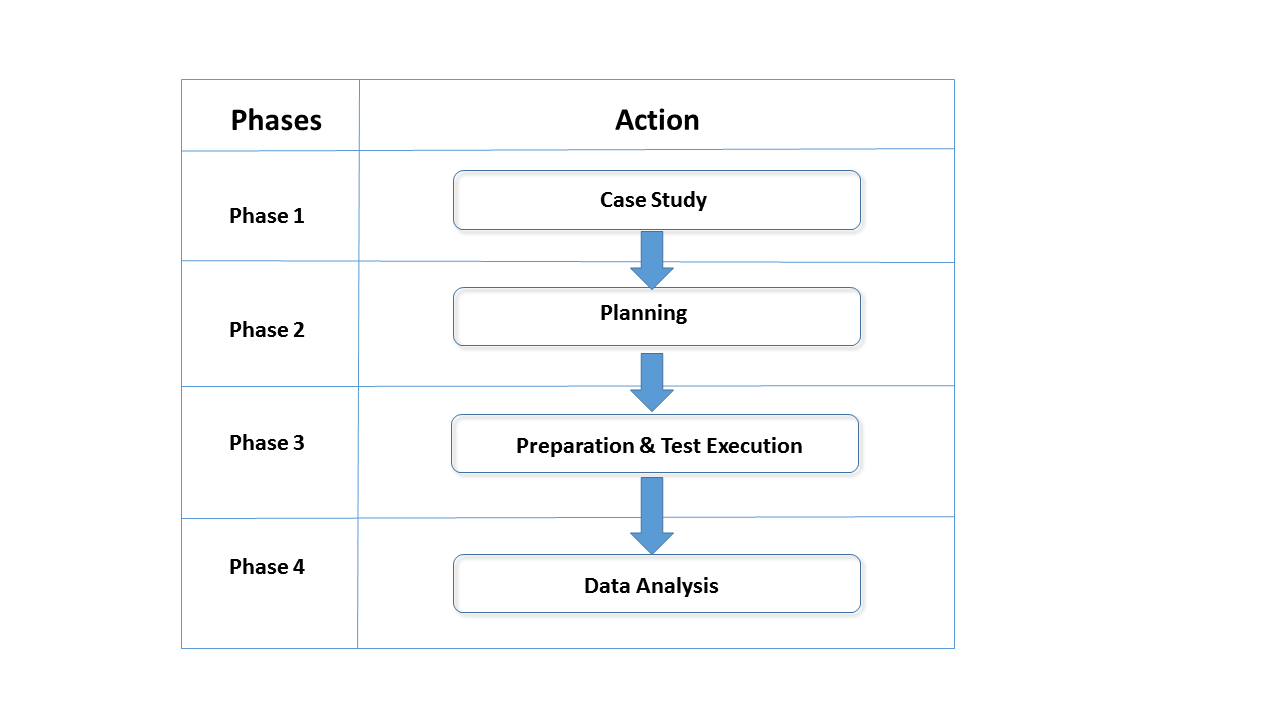
\includegraphics[width=1\textwidth]{figures/Evaluation_Phases}
	\caption{Evaluation Phases}
	\label{fig:Evaluation_Phases}
\end{figure}

\paragraph{Research Questions}
Our experience based on teaching and cooperation with industry has led us to suspect that people often draw their intuition for desired synchronisation behaviour directly from the special case of bijections.
This can be problematic and leads to statements such as: ``Why do I need a \emph{bidirectional} transformation language if the transformation at hand is not \emph{bijective}?''
Ironically, bidirectional transformation languages are often especially helpful when a transformation is \emph{not} bijective. As a sub-question of the research question \textbf{RQ 3} described earlier in Section \ref{subsec:contribution}, we propose to investigate if such misconceptions are really widespread or not:

\begin{description}
	\item[RQ 3.1 :] Do people tend to derive their (in general wrong) intuition for synchronisation scenarios from the special case of bijections?
\end{description}

To impart and train a more general intuition for synchronisation scenarios I have implemented \texttt{Demon-BX}, an online demonstrator for bidirectional transformations, as a platform for easily creating synchronisation scenarios to help achieve corresponding learning goals.
As a proof-of-concept, we have formulated five concrete learning goals, and designed corresponding scenarios based on a simple example. We believe (i) that example-based demonstrators are an effective way of achieving our (and similar) learning goals, and (ii) that a demonstrator is only useful in combination with carefully designed scenarios. As a sub-question of the research question \textbf{RQ 4} described earlier in Section \ref{subsec:contribution}, We propose to investigate these conjectures with the following two research questions: 

\begin{description}
	\item[RQ 4.1 :] Does demon-bx in combination with suitable scenarios support achieving corresponding learning goals?
	\item[RQ 4.2 :] How much does this support depend on the scenarios?  Would just playing with the demonstrator and the example already have an equal or comparably (positive) effect?
\end{description}

\paragraph{Purpose}
The purpose of the experiment is to evaluate whether it is possible to teach and enhance the understanding of the basic concepts of bx through the demonstrator.

\paragraph{Perspective}
The perspective is from the point of view of the researcher, i.e. the researcher would like to know if the usage of the demonstrator enhances the understanding of bx concepts of a user.

\paragraph{Context}
This experiment is on a bx tool demonstrator which falls under an educational environment and specifically under computer science branch. Hence, this experiment is mainly designed for the group of students/teachers/researchers from computer science area with or without prior knowledge of model driven software development field.

\subsection{Design Method}\label{subsec:designmethod} 
To investigate our research questions, I have used the Pretest-Posttest design method~\cite{analysisprepostdesigns}, a paired data analysis method in which the same experimental object is measured on some variables on two different occasions under different testing conditions. Here, I am using an extension of the Pretest-Posttest design method, called Pretest-Posttest control group design~\cite{expandquasiexpdesign}. It is a highly prestigious and one of the most popular research designs in use. The design principle is relatively simple, which involves two groups, a test group and a control group. First, the groups are pre-tested and then the test group is given the treatment. Afterward, both the groups are post-tested and data is collected from both occasions. Then, analysis is done by comparing pretest and posttest results collected from both the groups as explained in Figure~\ref{fig:PrePost_Test}.

\begin{figure}
	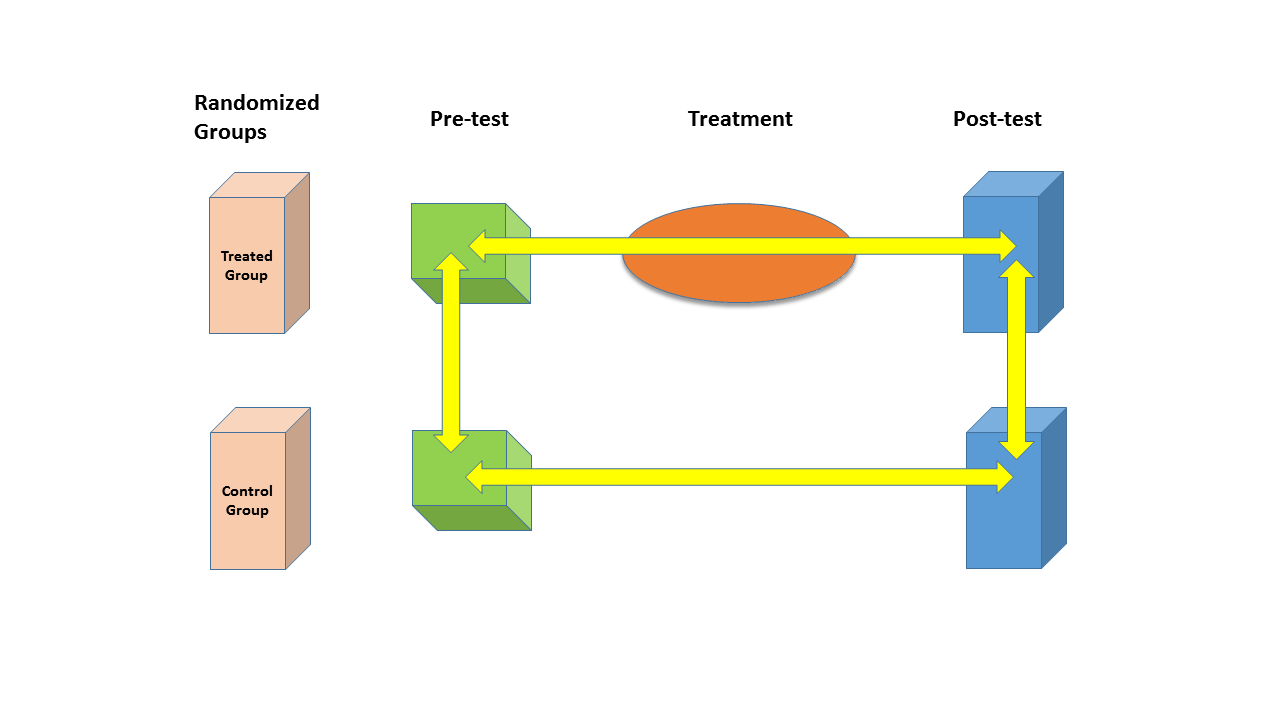
\includegraphics[width=1\textwidth]{figures/PrePost_Test}
	\caption{Pretest-Posttest Control Group Design }
	\label{fig:PrePost_Test}
\end{figure}

I have used this method because of the following reasons~\cite{anovapreposttest}:
\begin{itemize}
	\item It provides control over threats to internal validity.
	\item This allows the researchers to collect and compare posttest result from two groups, which give them an idea about the effectiveness of the treatment.
	\item The researcher can see how the groups have performed from pretest to posttest, whether one, both or neither improved over time.
\end{itemize}

In our case, we have designed test questions, one for each learning goal, to check if a participant has attained the learning goals or not.
We are also interested in the participants' subjective level of certainty for every given answer. 
The experiment is to be conducted as follows:

\begin{enumerate}
	\item All participants are divided randomly into two groups of equal size: the treated group and the control group.
	\item All participants take the pretest (answer all test questions).
	\item Both groups are allowed to use demon-bx for the same amount of time and are provided with an introduction and overview of the concrete example used in the demonstrator.
	The treated group is additionally provided with carefully chosen scenarios to work through, while the control group is not.
	\item When the time is up, all participants take the posttest (answer the same test questions again).
\end{enumerate}

\subsection{Planning}\label{subsec:planning}
\subsubsection{Participants}\label{subsubsec:participants}
As the context of the experiment is mainly focussed only on the computer science area, it will be conducted on a group of masters' student of computer science branch at Paderborn University. The participants are chosen based on convenience, i.e. the participants are the students taking a similar course.
\subsubsection{Hypotheses}\label{subsubsec:hypotheses} 

\subsubsection{Experimental Variables}\label{subsubsec:expvariables}

\paragraph{Independent Variables} The independent variables are listed below:

Does a group get scenarios to work through or not: nominal (yes or no)

\paragraph{Controlled Variables} The controlled variables are listed below:

Demonstrator platform: demon-bx\\
Concrete example: kitchen to grid\\
Group participants are chosen from: \{master students, PhD students, bx researchers, \ldots \}\\
Test questions\\
Learning goals\\
Max. time interval to answer questions: 55 min

\paragraph{Dependent Variables} The dependent variables are listed below:

Correctness score of pretest: ordinal\\
Correctness score of posttest: ordinal\\
Level of certainty of pretest:  ordinal\\
Level of certainty of posttest: ordinal

\subsubsection{Learning Goals \& Questions}\label{subsubsec:questions}
 
\subsection{Investigation of Goals}\label{subsec:investigationgoals} 

\subsection{Execution}\label{subsec:execution} 
\subsubsection{Preparation }\label{subsubsec:prep}
\subsubsection{Test Execution \& Data Collection}\label{subsubsec:execution&data}


\subsection{Threats to Validity and Mitigation}\label{subsec:threats&mitigation}

\subsection{Data Analysis and Results }\label{subsec:results}